\documentclass[conference]{IEEEtran}
\usepackage{url}
\usepackage{booktabs}
\usepackage{graphicx}
\usepackage{amsmath}
\usepackage{cite}

\title{GreenMind AI: A Multi-Metric Forecasting and Decision-Support Platform for Cloud GreenOps}
\author{\IEEEauthorblockN{Anonymous submission draft}}

\begin{document}
\maketitle

\begin{abstract}
Modern cloud operations require optimizing resource utilization, infrastructure cost, and environmental footprint simultaneously, yet predictive telemetry alone does not establish operational savings. This paper presents a comprehensive technical audit and architectural analysis of GreenMind AI, an open-source decision-support prototype for cloud GreenOps. The platform combines five one-hour-ahead machine learning forecasters with a five-domain multi-agent analysis engine (Cost, Performance, Sustainability, Security, and Reliability), transparent conflict arbitration, a non-destructive Digital Twin simulator, and an eight-tool explainable copilot. We evaluate the forecasting pipeline using the project's deterministic 60-day, 15-minute multi-metric synthetic dataset (5,756 chronological records) across a strict 80/20 train/test holdout (4,604 train and 1,152 test samples). GradientBoostingRegressor models achieve mean absolute error (MAE) improvements over a one-hour forecast-origin persistence baseline ranging from 25.4\% to 45.4\% across all five targets: CPU (3.809\% vs. 6.500\%), memory (2.979\% vs. 3.996\%), network (43.876 vs. 80.346~Mbps), cost (\$0.009 vs. \$0.013/h), and a synthetic carbon proxy (4.061 vs. 5.846~gCO$_2$/15-min). Our audit reveals that the stored rolling-mean baseline in the repository evaluates a one-step-ahead (15-minute) prediction on unshifted test data rather than a true four-step-ahead forecast from origin, which actually yields higher error (e.g., 7.263\% for CPU). Furthermore, we establish the boundaries of the system: the evaluations are derived from synthetic generator equations, cloud connector live behaviors are unverified end-to-end, and direct cloud remediation is strictly rejected at the API boundary with HTTP~501 (dry-run previews only). GreenMind AI provides an integrated software architecture for proactive cloud analysis, but synthetic accuracy must not be conflated with validated production cost or emission reductions.
\end{abstract}

\begin{IEEEkeywords}
Cloud computing, workload forecasting, gradient boosting, carbon-aware computing, synthetic telemetry, multi-agent systems, digital twin, decision support.
\end{IEEEkeywords}

\section{Introduction}
Cloud data centers consume substantial global electrical energy, driving both cloud providers and tenants toward carbon-aware computing and FinOps/GreenOps operational practices~\cite{r4},~\cite{r6}. Modern cloud management platforms expose multifaceted observability signals, spanning CPU and memory utilization, network bandwidth, hourly billing meters, and regional grid carbon-intensity feeds. Proactive workload forecasting can assist orchestrators in identifying resource bottlenecks, scheduling deferrable batch tasks, and planning right-sizing actions prior to demand spikes. However, high predictive accuracy on historical data does not inherently translate into realized financial savings, carbon abatement, or preserved service-level objectives (SLOs) in production systems~\cite{r3},~\cite{r8}.

In environmental accounting, estimating greenhouse gas emissions requires rigorous accounting boundaries, real-time power telemetry, facility Power Usage Effectiveness (PUE), and time-varying marginal emissions factors~\cite{r4},~\cite{r5}. Consequently, a synthetic or static proxy cannot be reported as an empirical Scope~2 carbon reduction without live meter verification. Similarly, automated remediation must balance conflicting operational trade-offs, such as performance headroom versus idle cost elimination.

GreenMind AI is an open-source software prototype developed to bridge the gap between predictive telemetry and operational decision support. The repository integrates a multi-metric forecasting pipeline, a FastAPI service layer, a TypeScript/React management cockpit, five domain-oriented analysis agents (Cost, Performance, Sustainability, Security, Reliability) orchestrated via a state graph, a deterministic conflict resolver, an eight-tool explainable copilot, and a non-destructive Digital Twin simulator. Connector modules exist for Amazon Web Services (AWS), Microsoft Azure, and Google Cloud Platform (GCP).

This paper delivers an empirical and architectural audit of the GreenMind AI implementation. We delineate three specific contributions:
\begin{enumerate}
    \item We detail the end-to-end software architecture linking multi-source telemetry ingestion, multi-metric gradient boosted forecasting, multi-agent arbitration, Digital Twin simulation, and decision-support copilot interfaces.
    \item We reproduce and verify the held-out forecasting performance across all five targets, analyzing feature importances and resolving a subtle baseline alignment discrepancy where stored moving averages reflected one-step-ahead predictions rather than four-step horizons.
    \item We explicitly demarcate the empirical evidence boundaries: demonstrating that reported gains stem from a deterministic synthetic generator, clarifying the carbon target definition, and documenting that live remediation is intentionally disabled via HTTP~501 to prevent unauthorized cloud mutations.
\end{enumerate}

\section{Related Work}
Workload and resource demand forecasting has evolved from classical statistical models to complex deep neural networks. Calheiros et al.~\cite{r7} demonstrated proactive cloud provisioning using autoregressive integrated moving average (ARIMA) models, showing that proactive scaling reduces QoS violations compared to reactive policies. Machine learning ensemble methods, particularly Friedman's Gradient Boosting Machine (GBM)~\cite{r1}, construct additive tree models that excel on tabular and structured lag features without demanding the compute scale of deep architectures. Recently, Rossi et al.~\cite{r3} investigated probabilistic LSTMs and Bayesian neural networks on Google and Alibaba cluster traces, highlighting that point forecasts fail to capture operational uncertainty and that transfer learning degrades across disparate cloud providers. GreenMind AI utilizes five lightweight GradientBoostingRegressor models; unlike~\cite{r3}, its evaluation is confined to synthetic series.

Evaluating time-series forecasters requires careful handling of temporal dependencies. Bergmeir, Hyndman, and Koo~\cite{r2} established that standard cross-validation can be theoretically valid for purely autoregressive models when errors are uncorrelated, but a single chronological holdout remains standard practice when simulating prospective deployment. GreenMind AI enforces an 80/20 chronological split to avoid forward-looking data leakage.

In green computing, Henderson et al.~\cite{r4} established systematic reporting standards for machine learning energy consumption and grid carbon footprints. Lannelongue, Grealey, and Inouye~\cite{r5} formulated the Green Algorithms framework, formalizing carbon calculations across runtime, TDP, PUE, and grid intensity. For hyperscale infrastructure, Radovanovic et al.~\cite{r6} deployed carbon-aware computing systems at Google datacenters using day-ahead predictions and Virtual Capacity Curves to temporally shift flexible workloads to cleaner grid hours. Dodge et al.~\cite{r8} measured operational carbon intensity across cloud instances, demonstrating that spatial region selection and temporal scheduling significantly reduce Scope~2 emissions. GreenMind AI incorporates regional intensity curves modeled after these principles, but applies them to synthetic telemetry rather than hardware meter feeds.

\section{Platform Architecture and Implementation}

\begin{figure*}[t]
\centering
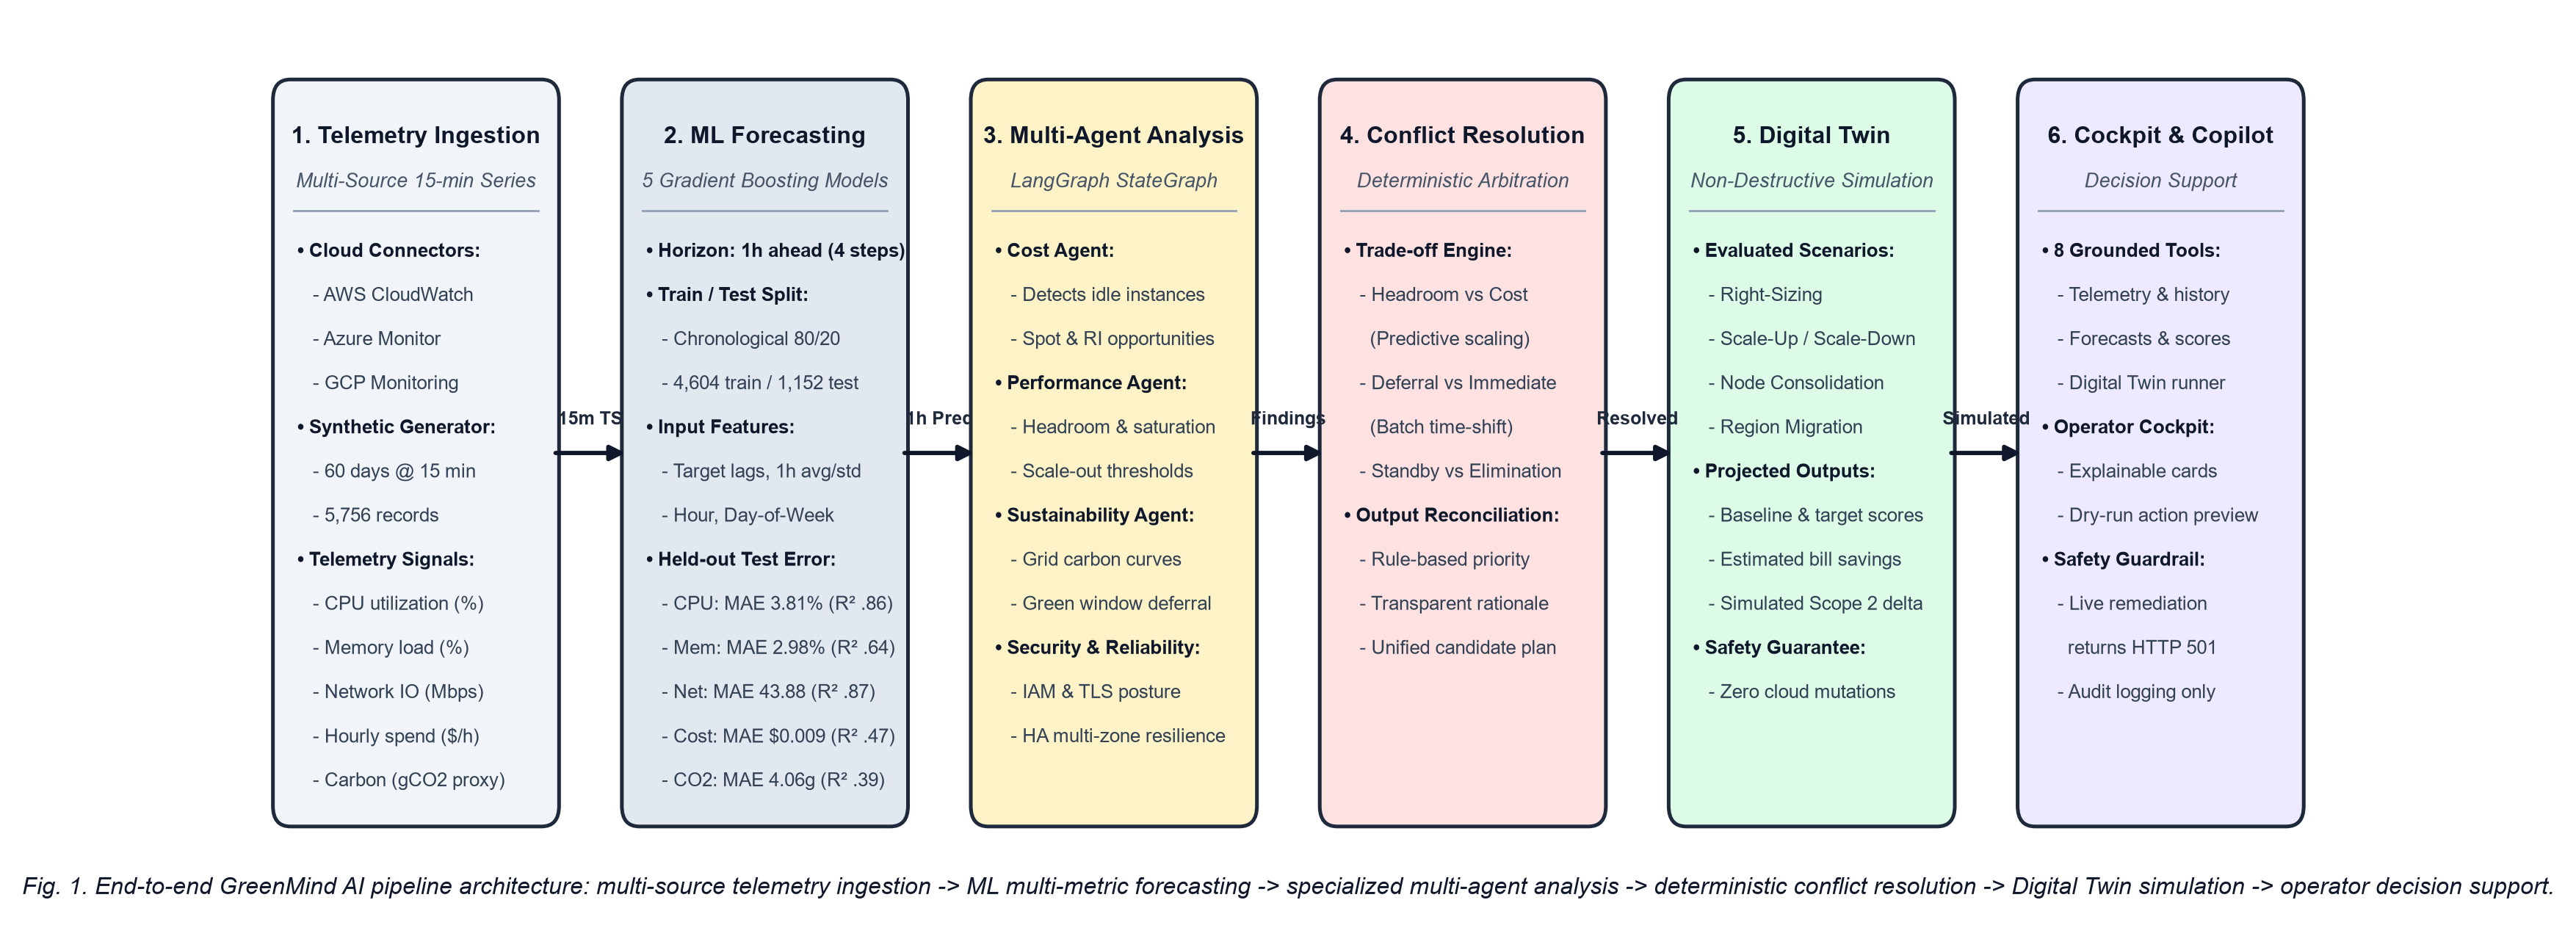
\includegraphics[width=0.98\textwidth]{greenmind_architecture.png}
\caption{End-to-end GreenMind AI pipeline architecture: multi-source telemetry ingestion $\rightarrow$ ML multi-metric forecasting $\rightarrow$ specialized multi-agent analysis $\rightarrow$ deterministic conflict resolution $\rightarrow$ Digital Twin simulation $\rightarrow$ operator decision support.}
\label{fig:arch}
\end{figure*}

The GreenMind AI architecture comprises six interconnected components, structured to prevent unauthorized cloud mutations while providing explainable operational intelligence (Fig.~\ref{fig:arch}).

\subsection{Telemetry Ingestion and Service Layer}
The backend service is implemented in FastAPI (Python 3.12) with SQLite/PostgreSQL persistence. Telemetry connectors interface with AWS CloudWatch (via \texttt{boto3}), Azure Monitor REST APIs, and GCP Cloud Monitoring v3. When valid credentials are not configured, each provider falls back to a deterministic synthetic generator. The system ingests five continuous signals at 15-minute intervals: CPU utilization (\%), memory load (\%), network traffic (Mbps), hourly compute spend (USD/h), and estimated carbon emissions proxy (gCO$_2$/15-min).

\subsection{Multi-Metric Machine Learning Predictor}
Five independent \texttt{GradientBoostingRegressor} models are trained for one-hour-ahead (four-step) forecasting. Each model is configured with 150 estimators, maximum tree depth of 3, learning rate of 0.08, and fixed random seed 42. Input features are structured to avoid forward lookahead:
\begin{itemize}
    \item \textbf{CPU, Memory, Network}: Current metric value $y_t$, cyclical timestamp indicators (hour of day, day of week), and backward-looking one-hour rolling mean and rolling standard deviation:
    \begin{equation}
        \mu_{t, 4} = \frac{1}{4} \sum_{i=0}^3 y_{t-i}, \quad \sigma_{t, 4} = \sqrt{\frac{1}{3} \sum_{i=0}^3 (y_{t-i} - \mu_{t, 4})^2}
    \end{equation}
    \item \textbf{Hourly Cost}: Current CPU, memory, cost ($y_t$), hour, and day of week.
    \item \textbf{Carbon Proxy}: Regional grid carbon intensity ($gCO_2/kWh$), hour, day of week, and CPU utilization.
\end{itemize}
Predictions are capped within physical bounds ($[0, 100]\%$ for CPU and memory). In \texttt{predictor.py}, an anomaly z-score threshold ($z > 2.5$) flags potential unexpected shifts against running metric statistics.

\subsection{Multi-Agent Analysis Engine}
Decision intelligence is partitioned into five specialized agents executed as a LangGraph \texttt{StateGraph}:
\begin{enumerate}
    \item \textbf{Cost Agent}: Evaluates spend rates, detects underutilized instances (CPU $< 10\%$), and recommends right-sizing, Spot instances, or 1-year Reserved Instances.
    \item \textbf{Performance Agent}: Monitors queue latency headroom, CPU/memory saturation, and flags when predictive scaling should trigger prior to a 75\% threshold.
    \item \textbf{Sustainability Agent}: Inspects 24-hour regional grid carbon-intensity curves and recommends deferring non-urgent batch jobs to clean energy windows (typically 1--6 AM UTC).
    \item \textbf{Security Agent}: Evaluates credential configuration, TLS enforcement, and IAM least-privilege policies.
    \item \textbf{Reliability Agent}: Assesses multi-zone redundancy, standby headroom, and automated backup schedules.
\end{enumerate}

\subsection{Deterministic Conflict Resolution}
When multiple agents generate opposing recommendations for the same resource, a deterministic arbitration engine reconciles the actions using explicit trade-off rules:
\begin{itemize}
    \item \textbf{Performance Headroom vs. Cost Optimization}: When CPU utilization is moderate ($35\% \le \text{CPU} < 75\%$) and Cost flags over-provisioning while Performance demands headroom, the engine approves right-sizing paired with predictive autoscaling, maintaining a 60-second scale-out buffer.
    \item \textbf{Reliability Standby vs. Cost Waste}: For idle standby instances ($\text{CPU} < 35\%$), the engine authorizes downsizing while keeping automated horizontal failover intact.
    \item \textbf{Carbon Deferral vs. Immediate Execution}: Non-urgent batch workloads are deferred to regional green windows, whereas critical interactive APIs remain untouched on immediate execution paths.
\end{itemize}
The conflict resolver emits an audit log detailing conflicting agents, competing proposals, reconciliation rationale, and an arbitration confidence score (typically $0.87$--$0.92$).

\subsection{Non-Destructive Digital Twin Simulator}
To evaluate operational impact without infrastructure risk, the Digital Twin engine simulates candidate actions against state snapshots. Supported scenarios include:
\begin{itemize}
    \item \textbf{Right-Sizing}: Projects downsized capacity on modern instance families, reducing estimated cost by 25\% and carbon by 20\%.
    \item \textbf{Scale-Up / Scale-Down}: Simulates horizontal replica adjustments and calculates resulting headroom changes.
    \item \textbf{Node Consolidation}: Simulates bin-packing low-utilization containers onto fewer physical nodes.
    \item \textbf{Region Migration}: Simulates shifting compute from carbon-heavy regions (e.g., \texttt{in-north}, $\sim$650~gCO$_2$/kWh) to hydroelectric grids (e.g., \texttt{ca-central}, $\sim$90~gCO$_2$/kWh).
\end{itemize}
The simulator recalculates a composite Optimization Score ($0$--$100$) before and after each scenario. All outputs are explicitly marked with the metadata flag \texttt{SIMULATED / ESTIMATED}.

\subsection{Copilot Tools and Safe Remediation Boundary}
An AI Cloud Copilot interfaces with operators through eight grounded tools: \texttt{get\_cloud\_metrics}, \texttt{get\_history}, \texttt{get\_predictions}, \texttt{get\_cost\_analysis}, \texttt{get\_carbon\_analysis}, \texttt{get\_recommendations}, \texttt{get\_cloud\_health}, and \texttt{run\_digital\_twin\_simulation}.
A critical safety boundary governs live remediation. In \texttt{backend/app/integrations/cloud\_actions.py}, non-dry-run remediation requests trigger an explicit HTTP~501 error:
\begin{quote}
\textit{HTTP 501: Live cloud remediation is not implemented. Use dry\_run=true to preview this action.}
\end{quote}
Rollback attempts likewise return HTTP~501. The system permits dry-run previews and persists simulated audit events, ensuring that no real cloud infrastructure mutation is executed.

\section{Experimental Methodology}

\subsection{Synthetic Telemetry Generation}
The synthetic generator in \texttt{generate\_dataset.py} creates 60 days of telemetry at 15-minute intervals starting June 1, 2026 ($N = 60 \times 96 = 5{,}760$ timestamps), using NumPy's default generator initialized with seed 42. Metrics are modeled using parameterized sinusoidal diurnal patterns:
\begin{equation}
    \text{CPU}_t = \text{clip}\left(35 + 30 \sin^2\left(\frac{h_t - 7}{24} 2\pi\right) \cdot W_t + \tau_t + \epsilon_t, 2, 98\right)
\end{equation}
where $h_t \in [0, 24)$ is the continuous hour, $W_t = 0.7$ on weekends and $1.0$ on weekdays, $\tau_t$ is a linear trend ($0$ to $5\%$), and $\epsilon_t \sim \mathcal{N}(0, 4^2)$. Memory load incorporates an upward drift ($0$ to $8\%$) representing memory leaks. Network traffic follows a diurnal curve centered at 9 AM ($300 + 400 \sin^2(\cdot)$ Mbps) with noise $\sigma = 50$. Hourly compute cost scales with CPU utilization based on an AWS \texttt{m5.xlarge} baseline (\$0.192/h).

\subsection{Carbon Target Formulation and Units}
The carbon target requires precise dimensional clarity. In \texttt{generate\_dataset.py}, regional carbon intensity $I(h_t)$ is looked up from an hourly profile for the \texttt{us-east} grid (ranging from 320 to 470~gCO$_2$/kWh). An assumed server power draw of $P = 0.35$~kW is integrated over the 15-minute time step ($\Delta t = 0.25$~h), yielding energy $E = 0.0875$~kWh. The target is defined as:
\begin{equation}
    C_t = \text{clip}\left(I(h_t) \cdot E + \mathcal{N}(0, 5^2), 0, 500\right)
\end{equation}
Thus, $C_t$ represents grams of CO$_2$ emitted per 15-minute observation step ($\text{gCO}_2/\text{15-min}$). The model predicts this quantity four steps ahead. This synthetic proxy excludes dynamic PUE variations, server fan curves, power supply losses, and embodied hardware emissions (Scope~3), distinguishing it from measured operational accounting.

\subsection{Chronological Holdout Protocol}
To model prospective forecasting without temporal leakage, observations are shifted by $\Delta t = 4$ steps ahead:
\begin{equation}
    y_t^{\text{target}} = y_{t+4}
\end{equation}
Dropping the trailing four rows without forward labels leaves $5{,}756$ complete records. The training script applies a strict chronological 80/20 partition: the first 4,604 observations (48 days) form the training set, and the final 1,152 observations (12 days) form the held-out test set. No row shuffling is performed.

\subsection{Baselines and Evaluation Measures}
Models are evaluated against two baseline predictors:
\begin{enumerate}
    \item \textbf{Persistence Baseline ($\hat{y}_{t+4} = y_t$)}: Predicts the target one hour ahead using the observation at the forecast origin $t$.
    \item \textbf{Rolling Mean Baseline}: In the repository's \texttt{baseline.py}, the evaluated baseline computes a four-sample moving average. Our audit identified that \texttt{evaluate\_rolling\_mean} predicts the next immediate step ($t+1$) on the unshifted test array ($N=1{,}148$), rather than projecting four steps ahead. We report both the stored baseline and the true four-step-ahead rolling baseline evaluated from forecast origin $t$.
\end{enumerate}

Evaluation metrics include Mean Absolute Error (MAE), Root Mean Squared Error (RMSE), Coefficient of Determination ($R^2$), and percentage MAE improvement over persistence:
\begin{equation}
    \text{Gain (\%)} = 100 \times \left(1 - \frac{\text{MAE}_{\text{model}}}{\text{MAE}_{\text{persistence}}}\right)
\end{equation}

\section{Experimental Results}

\begin{table*}[t]
\caption{Verified Evaluation Metrics on the Chronological Synthetic Test Set ($N=1{,}152$). Persistence Evaluates Metric Value at Forecast Origin $t$ Predicting $t+4$ (1~h Ahead). Stored Roll-4 Represents the Repository's Unshifted 1-Step Moving Average ($N=1{,}148$). True Roll-4 Evaluates the Origin Moving Average Predicting $t+4$.}
\label{tab:results}
\centering
\footnotesize
\begin{tabular}{lrrrrrrr}
\toprule
\textbf{Target Metric} & \textbf{Model MAE} & \textbf{Model RMSE} & \textbf{Model $R^2$} & \textbf{Persistence MAE} & \textbf{Stored Roll-4 MAE} & \textbf{True Roll-4 MAE} & \textbf{Gain over Pers. (\%)} \\
\midrule
CPU Utilization (\%) & 3.809 & 4.811 & 0.855 & 6.500 & 4.622 & 7.263 & 41.4\% \\
Memory Utilization (\%) & 2.979 & 3.704 & 0.636 & 3.996 & 3.025 & 4.153 & 25.4\% \\
Network Traffic (Mbps) & 43.876 & 55.328 & 0.871 & 80.346 & 56.727 & 90.816 & 45.4\% \\
Hourly Cost (USD/h) & 0.009 & 0.011 & 0.474 & 0.013 & 0.010 & N/A & 29.7\% \\
Carbon Proxy (gCO$_2$/15-min) & 4.061 & 5.087 & 0.391 & 5.846 & 4.571 & N/A & 30.5\% \\
\bottomrule
\end{tabular}
\end{table*}

Table~\ref{tab:results} reports the verified held-out performance across all five forecasting targets. All results were reproduced identically by executing \texttt{train.py} and audited via independent recomputation against the saved models.

Across all targets, the gradient boosted models outperform the forecast-origin persistence baseline on this synthetic holdout. Relative MAE improvements range from 25.4\% (memory) to 45.4\% (network). Network traffic and CPU utilization exhibit the highest goodness-of-fit ($R^2 = 0.871$ and $0.855$), reflecting the models' ability to capture the underlying sinusoidal generator rhythms.

Feature importance values extracted from the tree models explain the reliance on lag and cyclical inputs:
\begin{itemize}
    \item \textbf{CPU}: Current CPU lag dominates with 69.4\% importance, followed by hour of day (22.3\%), day of week (4.8\%), and rolling average (3.3\%).
    \item \textbf{Memory}: Current memory contributes 45.5\%, hour of day 35.7\%, and the one-hour rolling average 17.7\%.
    \item \textbf{Network}: Current network contributes 67.7\%, hour of day 26.0\%, and day of week 4.0\%.
    \item \textbf{Cost}: Driven primarily by CPU utilization (67.1\%) and hour of day (21.9\%), aligning with the generator formula where compute cost scales directly with active CPU load.
    \item \textbf{Carbon}: Dominated by regional grid carbon intensity (71.1\%), hour of day (20.0\%), and CPU utilization (8.5\%).
\end{itemize}

\section{Discussion and Technical Audit Findings}

\subsection{Baseline Alignment and Comparative Dynamics}
Our audit identified an important methodological nuance regarding the repository's rolling-mean baseline. The stored \texttt{rolling\_mae} in \texttt{metrics.json} evaluates $\hat{y}_{t+1} = \frac{1}{4} \sum_{i=0}^3 y_{t-i}$ on unshifted observations ($N=1{,}148$). Because cloud metrics possess high lag-1 autocorrelation in 15-minute synthetic intervals, this unshifted baseline predicts only 15 minutes ahead rather than the one-hour target horizon.

When evaluated as a true four-step-ahead baseline from origin $t$ (predicting $t+4$ using $\mu_{t,4}$), the baseline error increases significantly: CPU MAE rises from 4.622\% to 7.263\%, memory MAE from 3.025\% to 4.153\%, and network MAE from 56.727 to 90.816~Mbps. Under the correct horizon alignment, the true rolling-mean baseline performs worse than simple persistence (e.g., 7.263\% vs. 6.500\% for CPU) due to lag-induced phase shift during diurnal transitions. The gradient boosted models substantially outperform both persistence and the true rolling baseline.

\subsection{Predictive vs. Operational Realities}
While $R^2$ values for CPU (0.855) and network (0.871) are high, cost (0.474) and carbon (0.391) exhibit lower explained variance. For cost and carbon, the synthetic generator introduces Gaussian observation noise ($\sigma = 0.01$ and $\sigma = 5$) on small base values, creating an irreducible error floor on single-step targets.

More fundamentally, the models learn the smooth algebraic formulas programmed into \texttt{generate\_dataset.py}. Real cloud telemetry from hyperscale clusters (such as the Google and Alibaba traces analyzed in~\cite{r3}) features burstiness, heavy-tailed job distributions, sudden node preemptions, and non-stationary distribution shifts that do not follow sinusoidal curves. Consequently, performance on this synthetic generator does not establish generalization to production cloud workloads.

\section{Limitations and Threats to Validity}
Several limitations must be documented prior to academic consideration:
\begin{enumerate}
    \item \textbf{Data Provenance}: All reported evaluations originate from a single synthetic generator configuration (seed 42, 60 days, \texttt{us-east} curve). No public cluster traces or live cloud telemetry were evaluated.
    \item \textbf{Recursive Multi-Step Horizon Inconsistency}: In \texttt{predictor.py}, the \texttt{forecast\_multi\_step} wrapper recursively applies single-step updates at 5-minute intervals ($step \times 5$~min) using models trained directly on four-step (15-minute $\times$ 4 = 1-hour) shifts. Furthermore, predicted carbon ($gCO_2/15$-min, $\sim$30--40) is passed back into subsequent recursive steps as \texttt{carbon\_intensity}, which was trained on grid values ($gCO_2/kWh$, $\sim$350--450). This represents an out-of-distribution input during recursive multi-step extrapolation.
    \item \textbf{Unverified Live Connectors}: While connector classes exist for AWS, Azure, and GCP, live credential paths and telemetry polling were not validated across real cloud subscriptions for this paper.
    \item \textbf{Protected Cloud Mutation}: Live automated remediation is deliberately non-functional (HTTP~501). Simulated cost savings (\$864/month) and carbon reductions emitted by the Digital Twin represent static model projections, not realized financial or environmental outcomes.
    \item \textbf{Carbon Accounting Limitations}: The synthetic carbon target is an energy proxy assuming a constant 350~W server draw, omitting dynamic server power states, PUE variances, and embodied lifecycle emissions~\cite{r5}.
\end{enumerate}

\section{Conclusion and Future Work}
GreenMind AI implements a complete architectural prototype uniting multi-metric workload forecasting, multi-agent analysis, deterministic conflict arbitration, Digital Twin simulation, and copilot decision support. On a 60-day chronological synthetic benchmark, gradient boosted regressors reduce one-hour-ahead MAE by 25.4\% to 45.4\% compared to persistence. However, these results reflect synthetic generator learning rather than production cloud effectiveness. Future work must evaluate open cluster traces (e.g., Google Borg, Azure Functions), integrate real-time grid intensity feeds (Electricity Maps / WattTime), resolve recursive multi-step horizon alignment, and conduct end-to-end live testing with isolated canary infrastructure before autonomous operational claims can be substantiated.

\begin{thebibliography}{00}
\bibitem{r1} J. H. Friedman, ``Greedy function approximation: A gradient boosting machine,'' \emph{The Annals of Statistics}, vol. 29, no. 5, pp. 1189--1232, Oct. 2001, doi: 10.1214/aos/1013203451.
\bibitem{r2} C. Bergmeir, R. J. Hyndman, and B. Koo, ``A note on the validity of cross-validation for evaluating autoregressive time series prediction,'' \emph{Computational Statistics \& Data Analysis}, vol. 120, pp. 70--83, Apr. 2018, doi: 10.1016/j.csda.2017.11.003.
\bibitem{r3} A. Rossi, A. Visentin, D. Carraro, S. Prestwich, and K. N. Brown, ``Forecasting workload in cloud computing: Towards uncertainty-aware predictions and transfer learning,'' \emph{Cluster Computing}, vol. 28, art. no. 258, pp. 1--22, 2025, doi: 10.1007/s10586-024-04933-2.
\bibitem{r4} P. Henderson, J. Hu, J. Romoff, E. Brunskill, D. Jurafsky, and J. Pineau, ``Towards the systematic reporting of the energy and carbon footprints of machine learning,'' \emph{Journal of Machine Learning Research}, vol. 21, no. 248, pp. 1--43, 2020.
\bibitem{r5} L. Lannelongue, J. Grealey, and M. Inouye, ``Green algorithms: Quantifying the carbon footprint of computation,'' \emph{Advanced Science}, vol. 8, no. 12, art. no. 2100707, pp. 1--10, 2021, doi: 10.1002/advs.202100707.
\bibitem{r6} A. Radovanovic, R. Koningstein, I. Schneider, B. Chen, A. Duarte, B. Roy, D. Xiao, M. Haridasan, P. Donohoe, N. de M. L. Jacob, P. Douglis, and W. D. Weihl, ``Carbon-aware computing for datacenters,'' \emph{IEEE Transactions on Power Systems}, vol. 38, no. 2, pp. 1270--1280, Mar. 2023, doi: 10.1109/TPWRS.2022.3173250.
\bibitem{r7} R. N. Calheiros, E. Masoumi, R. Ranjan, and R. Buyya, ``Workload prediction using ARIMA model and its impact on cloud applications' QoS,'' \emph{IEEE Transactions on Cloud Computing}, vol. 3, no. 4, pp. 449--458, Oct.--Dec. 2015, doi: 10.1109/TCC.2014.2350475.
\bibitem{r8} J. Dodge, T. Prewitt, R. T. Des Combes, E. Odmark, R. Schwartz, E. Strubell, A. S. Luccioni, N. A. Smith, N. DeCario, and W. Buchanan, ``Measuring the carbon intensity of AI in cloud instances,'' in \emph{Proceedings of the 2022 ACM Conference on Fairness, Accountability, and Transparency (FAccT '22)}, Seoul, Republic of Korea, 2022, pp. 1536--1546, doi: 10.1145/3531146.3533147.
\bibitem{r9} Pratham-stack-coder, ``GreenMind-AI repository,'' GitHub, 2026. [Online]. Available: \url{https://github.com/Pratham-stack-coder/GreenMind-AI}.
\end{thebibliography}

\end{document}
